\section{原理}

\subsection{脉冲产生}

\begin{figure}[htbp]
	\centering
	\begin{minipage}[t]{0.48\textwidth}
		\centering
		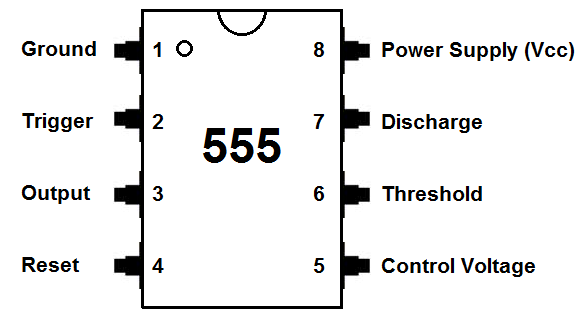
\includegraphics[width=6cm]{figure/LM555.png}
		\caption{外部引脚图}\label{fig:LM555}
	\end{minipage}
	\begin{minipage}[t]{0.48\textwidth}
		\centering
		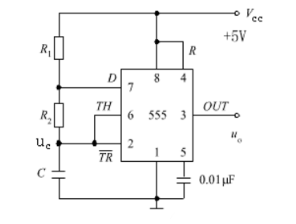
\includegraphics[width=6cm]{figure/LM555_circuit.png}
		\caption{电路原理图}\label{fig:LM555 circuit}
	\end{minipage}
\end{figure}

利用 555 电路组成触发器,利用电容的充放电原理产生方波脉冲信号,通过调节电容的大小来控制输出脉冲的频率,输出频率计算公式为 $f=\frac{1.43}{(R_1+2R_2)C}$,利用触发器产生 1 Hz 的脉冲,实际周期为 0.984 秒,误差在可接受范围内,555 定时器的外部引脚图如图 \ref{fig:LM555} 所示,表 \ref{LM555} 展示了对应功能。

\begin{table}[hbtp]
	\setlength{\abovecaptionskip}{0cm} 
	\setlength{\belowcaptionskip}{-0.2cm}
	\begin{center}
	\caption{引脚功能表}
	\begin{tabular}{|c|c|p{10cm}|}
		\hline
		\textbf{引脚} & \textbf{名称} & \multicolumn{1}{c|}{\textbf{功能}}                              \\ \hline
		1           & GND(地)      & 接地,作为低电位(0V)                             \\ \hline
		2           & TRIG(触发)    & 当此引脚电压降至1/3VCC(或由控制端决定的阈值电压)时输出端给出高电位。   \\ \hline
		3           & OUT(输出)     & {\color[HTML]{000000} 输出高电平(+VCC)或低电位。}  \\ \hline
		4           & RST(复位)     & 当此引脚接高电平时定时器工作,当此引脚接地时芯片复位,输出低电位。        \\ \hline
		5           & CTRL(控制)    & 控制芯片的阈值电压(当此管脚接空时默认两阈值电压为1/3VCC与2/3VCC)。 \\ \hline
		6           & THR(阈值)     & 当此引脚电压升至2/3VCC(或由控制端决定的阈值电压)时输出端给出低电位。   \\ \hline
		7           & DIS(放电)     & 内接OC门,用于给电容放电。                           \\ \hline
		8           & VCC(供电)     & 提供高电位并给芯片供电。                             \\ \hline
	\end{tabular}\label{LM555}
	\end{center}
\end{table}


电容放电所需时间

\begin{equation}
t_2=R_2C\ln \frac{0-2/3V_{cc}}{0-1/3V_{cc}}=R_2C\ln 2\approx 0.7R_2C
\end{equation}

电容充电时间

\begin{equation}
t_1=\left( R_1+R_2 \right) C\ln \frac{V_{cc}-1/3V_{cc}}{V_{cc}-2/3V_{cc}}=\left( R_1+R_2 \right) C\ln 2\approx 0.7\left( R_1+R_2 \right) C
\end{equation}

电路频率 $f=\frac{1}{t_1+t_2}=\frac{1.43}{\left( R_1+2R_2 \right) C}$,而 $R_1=R_2=10\mathrm{k}\Omega $,故 $C=47\mathrm{\mu F}$。


\begin{figure}[htbp]
	\centering
	\begin{minipage}[t]{0.48\textwidth}
		\centering
		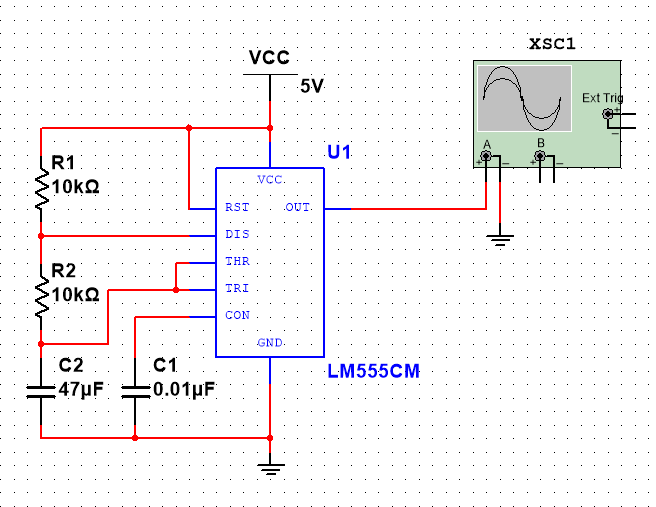
\includegraphics[width=6cm]{figure/signal1.png}
		\caption{脉冲信号产生电路图}\label{fig:signal1}
	\end{minipage}
	\begin{minipage}[t]{0.48\textwidth}
		\centering
		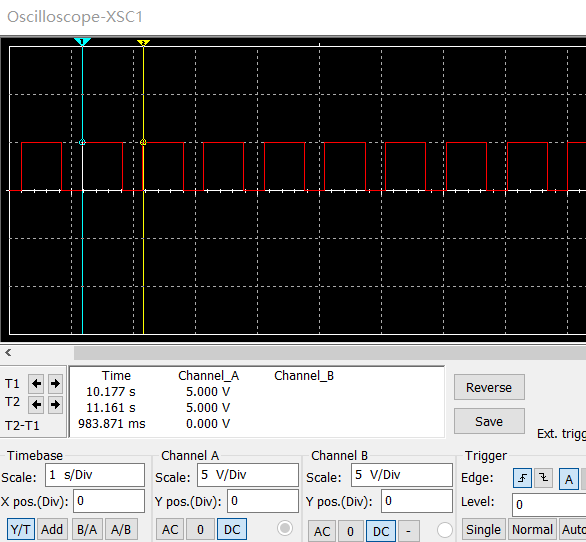
\includegraphics[width=6cm]{figure/signal2.png}
		\caption{脉冲信号波形图}\label{fig:signal2}
	\end{minipage}
\end{figure}

\subsection{计时}

用于计时的主体芯片为 7 块 74160N,分别用来对星期、时、分、秒进行计数。

\subsubsection{分与秒的计数}

分与秒都是 60 进制(0-59),它们的电路基本相同,60 进制计数器采用两块 74160N \textbf{整体置 0 法} 来实现。设计的电路图如图 \ref{fig:minute} 和图 \ref{fig:second} 所示。

\begin{figure}[htbp]
	\centering
	\begin{minipage}[t]{0.48\textwidth}
		\centering
		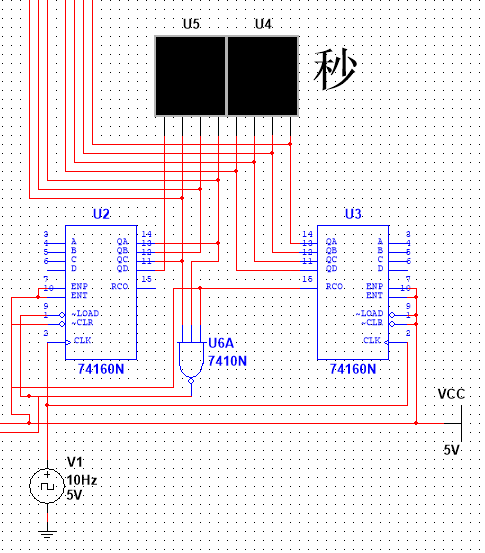
\includegraphics[width=6cm]{figure/second.png}
		\caption{秒的计数电路图}\label{fig:second}
	\end{minipage}
	\begin{minipage}[t]{0.48\textwidth}
		\centering
		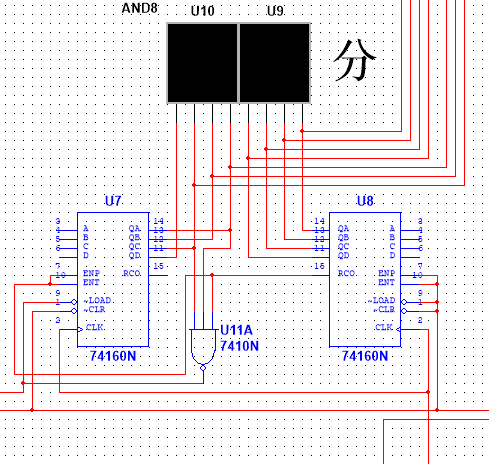
\includegraphics[width=6cm]{figure/minute.png}
		\caption{分的计数电路图}\label{fig:minute}
	\end{minipage}
\end{figure}

\subsubsection{时的计数}

时是 24 进制(0-23),24 进制计数器采用两块 74160N \textbf{整体置 0 法}来实现。设计的电路图如图 \ref{fig:hour} 所示。

\begin{figure}[hbtp]
	\centering
	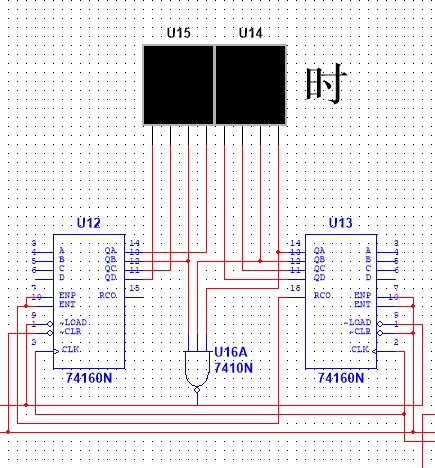
\includegraphics[width=6cm]{figure/hour.png}
	\caption{时的计数电路图}\label{fig:hour}
\end{figure}

\subsubsection{星期的计数}

我用 DCD\_HEX\_GREEN 上的 8 来表示周日,那么周是 7 进制(0-6),7 进制计数器为 0 时利用一个或非门电路转化为 8 也就是周日,采用一块 74160N 来实现。设计的电路图如图 \ref{fig:week} 所示。

\begin{figure}[hbtp]
	\centering
	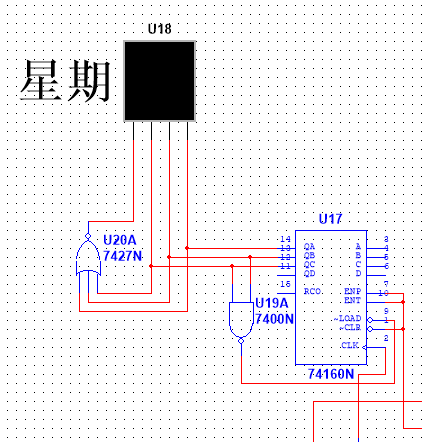
\includegraphics[width=6cm]{figure/week.png}
	\caption{星期的计数电路图}\label{fig:week}
\end{figure}

\subsection{显示}

通过将计数部分的四个输出端即 74160N 的输出端 $Q_A$、$Q_B$、$Q_C$、$Q_D$ 送入对应显示模块的输入端来使显示模块显示相应的数字,显示模块用了 DCD\_HEX\_BLUE(时分秒) 和 DCD\_HEX\_GREEN(星期)。

\subsection{校准}

校准包括星期校准、时校准、分校准三个部分。通过按下对应校准开关进行校准,原理是星期、时、分分别输入 5Hz、10Hz、50Hz时钟信号进行校准,实际应用中可根据实际情况进行修改,为防止校准信号丢失,利用了 RS 触发器电路,来提高电路的稳定性。校时电路的基本构造如图 \ref{fig:checkout} 所示。

\begin{figure}[hbtp]
	\centering
	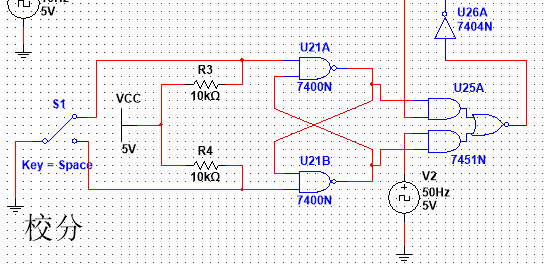
\includegraphics[width=6cm]{figure/checkout.png}
	\caption{校时电路的电路图}\label{fig:checkout}
\end{figure}

\subsection{报时}

整点报时电路要求在每个整点前鸣叫 5 次低音(500Hz),即在 59 分 50 秒到 59 分 59 秒之间,从 59 分 50 秒开始蜂鸣器每隔 1 秒响一次,最后在整点鸣叫一次高音(1000Hz),可以用门电路的与实现,分别如图 \ref{fig:Buzzer500Hz} 和图 \ref{fig:Buzzer1000Hz} 所示,500Hz 蜂鸣器连 7 个引脚,即分计数器十位的 $Q_C$ 和 $Q_A$、分计数器个位的 $Q_D$ 和 $Q_A$、秒计数器十位的 $Q_C$ 和 $Q_A$ 以及秒计数器个位的 $Q_A$ 的取反。

\begin{figure}[htbp]
	\centering
	\begin{minipage}[t]{0.48\textwidth}
		\centering
		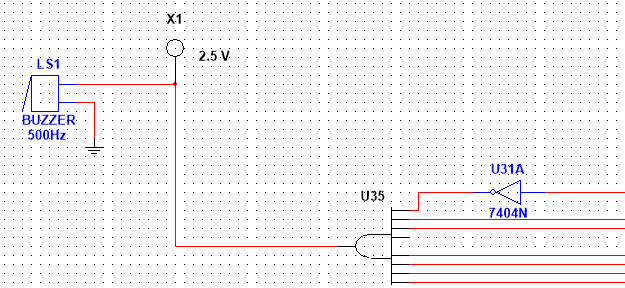
\includegraphics[width=6cm]{figure/Buzzer_500Hz.png}
		\caption{500Hz峰鸣器门电路图}\label{fig:Buzzer500Hz}
	\end{minipage}
	\begin{minipage}[t]{0.48\textwidth}
		\centering
		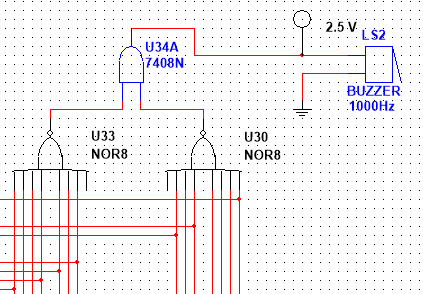
\includegraphics[width=6cm]{figure/Buzzer_1000Hz.png}
		\caption{1000Hz蜂鸣器门电路图}\label{fig:Buzzer1000Hz}
	\end{minipage}
\end{figure}